\section{Reconnecting the Loop}

The three collapses can reinforce one another. A weakened professional position makes immediate recognition elsewhere more attractive. A feedback environment that rarely tests judgment supplies less practice in calibration. Reduced confidence and fewer usable alternatives can make it harder to regain an effective position.

This is a possible reinforcing loop, with identifiable mechanisms and points of intervention. The book's diagnosis becomes useful when each connection can be investigated separately.

\subsection{Three Clocks, Several Interventions}

Job structures can change over years. Interfaces can change within weeks. Skills, habits, and relationships develop on varied timescales and can continue changing throughout adult life. Assigning agency recovery an immutable generational clock would obscure opportunities to improve it now.

A simple recurrence can illustrate declining entry costs into a replacement experience:
\begin{equation}
 c_{n+1}=Gc_n,\qquad
 G=g_1g_2g_3.
\end{equation}
If the $g_i$ are positive cost multipliers below one, the modeled cost decreases over repeated cycles. The recurrence describes its defined cost. It does not establish the stability, speed, or inevitability of the entire social loop.

A fuller account would need separate state variables for position, feedback, and agency, as well as delays and outside inputs. Evidence must show that one change actually strengthens the next. Those tests turn a suggestive diagram into an investigated mechanism.

Measurements can begin with narrower questions. Has entry into a profession become harder? Does assistance improve independently tested skill or only immediate output? Can users identify and challenge a consequential error? Do appeals change decisions? Are alternatives affordable and usable?

No single dashboard answers them all. Quantitative measures can be combined with longitudinal studies, task tests, institutional records, and specific cases. The possibility of gaming a measure is a reason to design review, rather than abandon measurement altogether.

\subsection{Four Functions of an Accountability System}

Consequences need a route into response. Four functions supply it:

\textbf{Discovery.} A system needs ways to detect harm, near misses, and material departures from expected behavior. Users and affected people need a reporting channel as well as operators' monitoring.

\textbf{Traceability.} Investigators need enough information to connect an event to relevant decisions, versions, configurations, and tool actions. Records should be proportionate, secure, and governed by privacy and access rules.

\textbf{Loss containment.} Someone must have usable authority to interrupt, isolate, recall, or otherwise limit continuing damage. Emergency containment may precede a full causal explanation.

\textbf{Remedy.} An affected person needs a practical route to correction, compensation where appropriate, and prevention of recurrence. Financial capacity matters because an obligation with no resources behind it may offer little relief.

These functions interact and can run concurrently. They are more demanding than a list of promised safeguards because each requires an actor, resources, and an operational interface.


\begin{figure}[ht]
\centering
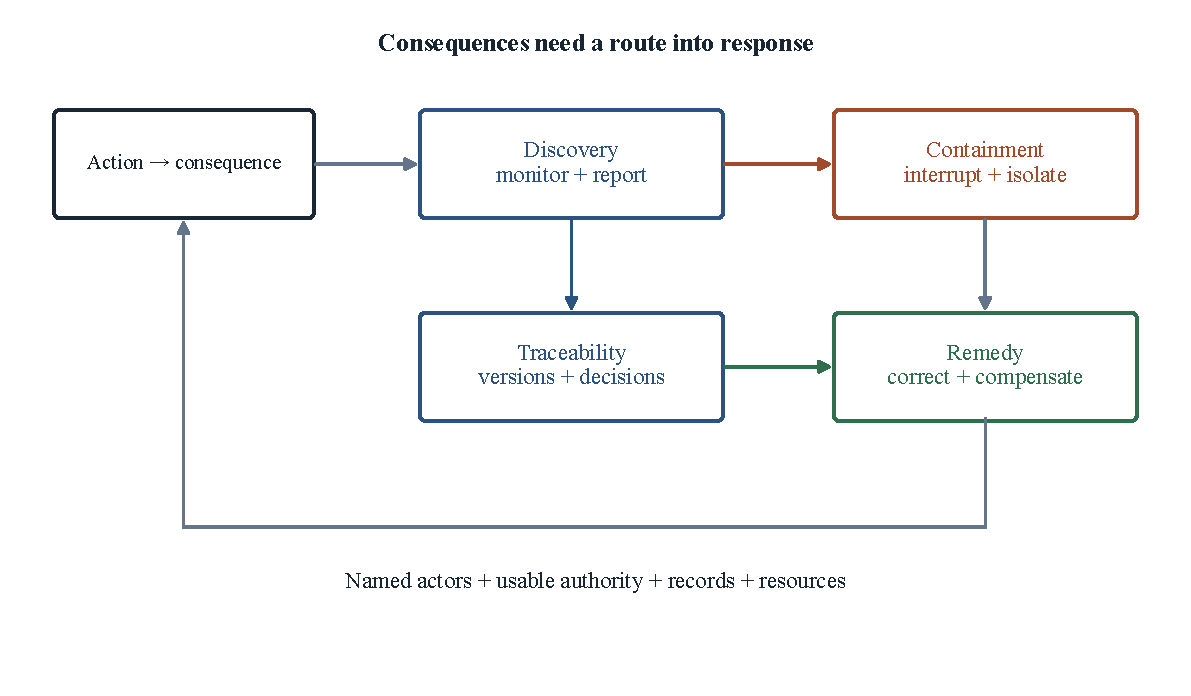
\includegraphics[width=\textwidth]{assets/accountability.pdf}
\caption{Accountability needs named actors, usable authority, records, and resources. Discovery, traceability, containment, and remedy can proceed concurrently, with their results feeding back into action.}
\label{fig:mechanism-accountability}
\end{figure}
Civil aviation is a familiar architecture in which design assurance, production controls, maintenance, operational authority, reporting, and investigation combine. Its reliability comes from aircraft and institutions together. Different domains need their own arrangements rather than a copied checklist.

Machine systems need the same clarity at their own interfaces. Which entity controls the update? Who can suspend access? Which records survive a service shutdown? Who can contest a model-based decision? Which party can fund a remedy?

Allocation can follow control, contractual role, statutory duty, or other legally established criteria. Insurance and compensation funds can pool some losses. Independent investigation can help distinguish learning from immediate fault allocation. None of these mechanisms works automatically; incentives and enforcement determine whether the promised function exists in practice.

The policy cost is visible now. The avoided harm is uncertain and later. Institutions are needed partly because the party paying for a safeguard may capture only a fraction of its benefit.

Accountability can also expand deployment. A risk with identified controls, records, and remedies is easier to evaluate than a risk that vanishes into a chain of disclaimers. Some uncertainty becomes manageable because the system now knows what it will do when uncertainty becomes consequence.

\subsection{Judgment Needs Standing}

Three decisions remain central: which consequences are acceptable, how much evidence is enough to proceed, and who may impose a cost on whom.

Models can inform all three. They can estimate outcomes, compare options, reveal inconsistencies, and help people articulate positions. Technical competence alone does not supply the right to decide.

The normative principle advanced here is that people bearing consequences must retain effective voice, representation, and access to challenge. Direct exposure is one source of standing; lawful delegation, professional duty, democratic authorization, and protections for absent or vulnerable parties are others.

A judge's, clinician's, or juror's authority depends on an institutional role and duties owed to others. The responsibility of a professional and the bodily risk borne by a patient remain distinct.

Jury systems illustrate one institutional choice about participation and judgment \cite{kalven1966american}. Their justification rests on the role, procedure, and distribution of public power. Medical consent illustrates another: expertise informs the options while the patient retains rights over exposure. Aviation assigns operational authority through defined roles, competence, and duties.

The common achievement is a decision with an intelligible basis, a recognized scope, and a place where it can be questioned. An opaque recommendation becomes a legitimate decision only through such an arrangement.

\subsection{A Person's Worth Survives a Falling Production Cost}

A society that values people only through scarce output becomes vulnerable when output becomes abundant. It needs a richer account of participation, care, relationship, judgment, and finite life.

The fact that a consequence happens to fall on someone does not justify making them bear it. Exposure creates a claim to protection and voice, rather than a duty to suffer for meaning. Responsibility should follow a justified allocation of authority and control.

Some parts of life remain personal in a direct sense. Another person can advise, work, or decide on one's behalf. They cannot thereby live the same finite life or occupy the same relation. Assistance changes what a person can do; it does not make the person's stake disappear.

The chapter's repair is therefore structural and concrete. Rebuild routes into useful contribution. Preserve feedback that can correct a claim. Keep exit, objection, and meaningful commitments available. Attach consequential action to people and institutions able to answer for it.

These choices create costs. The next chapter asks how to distinguish the costs that merely obstruct from those that preserve the conditions under which progress remains worth having.
